\documentclass[crop=false,10pt]{standalone}
\usepackage{standard}

\begin{document}
  \section{The Model} % (fold)
  \label{sec:The Model}
    \begin{figure*}[h]
      \center
      \begin{subfigure}[c]{0.49\textwidth}
        \center
        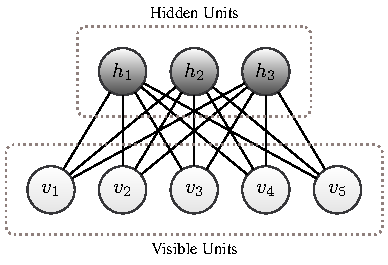
\includegraphics[scale=1]{figures/rbm-scheme-inputs.pdf}
      \end{subfigure}
      \begin{subfigure}[c]{0.49\textwidth}
        \center
        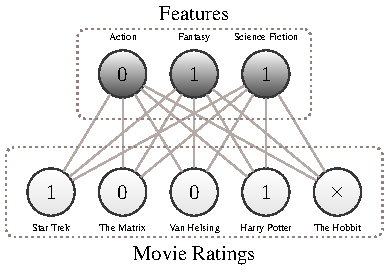
\includegraphics[scale=1]{figures/rbm-scheme-example.pdf}
      \end{subfigure}
      \caption{%
        Figure for scheme and example!
      }
      \label{fig:rbm-scheme-and-example}
    \end{figure*}
    To understand the model of an RBM let us first consider the general idea by looking at the left part of figure \ref{fig:rbm-scheme-and-example}.
    It shows a simple schematic example of an RBM.
    At first sight there seems to be no real difference to a standard feed-forward neural network (FFNN) with two layers.
    For an RBM every edge is undirected.
    Therefore the influence of one neuron to another cannot be computed directly as one maybe used to be in the FFNN.

    Apart from this subtle difference there are two obvious properties which are defining the RBM.
    First, the neurons in the RBM are separated into two subsets, the hidden units and the visible units.
    And second, connections between neurons via edges are only allowed between those two subsets.

    Based on these properties there is no real obvious interpretation for values of these units.
    But we have to remember that we want to model a probability distribution.
    So we will interpret every unit as input value for our RBM.
    Looking at the right part of figure \ref{fig:rbm-scheme-and-example} it is shown applied on the movie ratings from a user.
    Every rating from one user can be seen as a visible value.
    Based on these visible values an RBM can assign some hidden values based on some learned features, like movie genres \enquote{Action} or \enquote{Fantasy}.
    These hidden values for example would describe if the user likes the movie genre.

    Because we want to model the probability distribution with the given undirected bipartite graph, we first have to define some parameters.
    Here we can choose the standard approach of introducing biases for every neuron and weights for every edge.
    Therefore we get two bias vectors for the hidden and visible values and one weight matrix.
    Figure \ref{fig:rbm-scheme} shows schematically.
    \begin{figure}[H]
      \center
      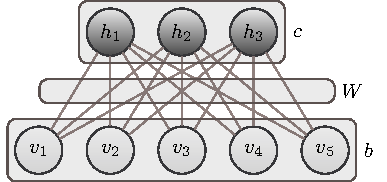
\includegraphics[width=0.441\textwidth]{figures/rbm-scheme.pdf}
      \caption{%
        The figure shows the basic scheme of an RBM with the weight matrix $W$ and bias vectors $b$ and $c$ as parameters describing the probability distribution modelled by the RBM.
      }
      \label{fig:rbm-scheme}
    \end{figure}

    To be precise, we will first define the sets for the input parameters.
    \[
      v \in V \define \set{0,1}{}^n
    \]
    \[
      h \in H \define \set{0,1}{}^m
    \]
    The parameters describing the RBM are taken to be real.
    We will abbreviate the weight matrix and the two bias vectors as one parameter.
    This will make the following formulas much more readable.
    \[
      ϑ \define (W,b,c) \in \setReal^{(n\times m) + n + m}
    \]

    Now we will define the probability distribution the RBM is modelling with respect to its parameters.
    This is a definition and not a corollary.
    Of course, we could choose another approach.
    But this would not be a RBM.
    \[
      \function{p[ϑ]}{V\times H}{[0,1]}
    \]
    \[
      p[ϑ](v,h) \define \frac{e^{ -E[ϑ](v,h) }}{Z(ϑ)}
    \]
    Here we define $E[ϑ]$ to be the so called energy function of the RBM.
    We have already introduced non-linearity by the exponential function.
    Therefore one chooses $E[ϑ]$ as simple as possible.
    \[
      \function{E[ϑ]}{V\times H}{\setReal}
    \]
    \[
      E[ϑ](v,h) \define -\transpose{v}Wh - \transpose{v}b - \transpose{h}c
    \]
    For completeness the normalization will be supplied.
    The definition for $Z(ϑ)$ is straightforward and not important for the learning or inference processes.
    \[
      Z(ϑ) \define \sum_{v\in V} \sum_{h\in H} e^{ -E[ϑ](v,h) }
    \]
    At this point one could think, that major problem in our model.
    If we cannot observe hidden values then how should we able to model a probability distribution over them.
    We can omit this problem by defining the probability distribution for the visible values.
    \[
      \function{p[ϑ]}{V}{[0,1]}
    \]
    \[
      p[ϑ](v) \define \sum_{h\in H} p[ϑ](v,h)
    \]
    This is the complete description of our model.
    But because of the two main properties of an RBM we can derive an important equation which will enable us to learn an RBM and to do some inference.
    \[
      p[ϑ](h \vert v) = \prod_{j=1}^m p[ϑ]\roundBrackets{h_j=1 \middle\vert v}
    \]
  % section The Model (end)
\end{document}